\subsection{Stored Procedures for Data Retrieval}

This section presents stored procedures used to retrieve meaningful information from the database. 
Unlike the procedures in Section 2.1, these procedures do not modify data. 
Instead, they support searching, filtering, joining related tables, aggregation, grouping, and sorting results for the application interface.

The first procedure retrieves games by genre and maximum price. 
The second procedure retrieves developers whose revenue exceeds a given threshold within a selected date range. 
Together, these procedures demonstrate how stored procedures can support realistic data retrieval operations in a Steam-like digital distribution platform.
\subsubsection{Procedure 1: Get Games by Genre and Price}

The procedure \texttt{GetGamesByGenreAndPrice} retrieves games that belong to a selected genre and have a base price not greater than a given maximum price. 
This procedure is similar to a filtering feature in a digital game store, where users can browse games by category and price range.

The procedure joins the \texttt{GAME}, \texttt{GAME\_GENRE}, and \texttt{DEVELOPER} tables. 
The parameter \texttt{p\_GenreName} is used to filter games by genre, while \texttt{p\_MaxPrice} limits the result to games whose base price does not exceed the selected value. 
The result is ordered by base price in descending order and then by game title in ascending order.

\begin{lstlisting}[language=SQL, caption={Procedure for retrieving games by genre and maximum price (column aliases shown in English; the actual SQL file in \texttt{SQLData/Procedure1.sql} uses Vietnamese aliases for end-user display)}, label={lst:get-games-by-genre-price}]
DELIMITER $$

CREATE PROCEDURE GetGamesByGenreAndPrice(
    IN p_GenreName VARCHAR(50),
    IN p_MaxPrice DECIMAL(10,2)
)
BEGIN
    SELECT
        g.game_id,
        g.title        AS `Game Title`,
        g.base_price   AS `Base Price`,
        g.release_date AS `Release Date`,
        d.legal_name   AS `Developer`
    FROM `GAME` g
    JOIN `GAME_GENRE` gg ON g.game_id = gg.game_id
    JOIN `DEVELOPER`  d  ON g.developer_id = d.user_id
    WHERE gg.genre_name = p_GenreName
      AND g.base_price <= p_MaxPrice
    ORDER BY g.base_price DESC, g.title ASC;
END$$
\end{lstlisting}
\subsubsection{Procedure 2: Get Developer Revenue}

The procedure \texttt{GetDeveloperRevenue} retrieves developers whose total revenue is greater than or equal to a given threshold within a selected date range.
This procedure supports the developer-side view of the platform, where developers or administrators may want to analyze sales performance.

The procedure calculates revenue from sold games by joining the \texttt{DEVELOPER}, \texttt{GAME}, \texttt{CONTAINS}, and \texttt{TRANSACTION} tables.
It uses two aggregate functions, \texttt{COUNT(c.game\_id)} for the total number of sold copies and \texttt{SUM(c.price\_at\_purchase)} for the total revenue, groups the result by developer, filters developers using the \texttt{HAVING} clause (\texttt{SUM(c.price\_at\_purchase) >= p\_MinRevenue}), and orders the output by total revenue in descending order.

\begin{lstlisting}[language=SQL, caption={Procedure for retrieving developer revenue (column aliases shown in English; the actual SQL file uses Vietnamese aliases such as \texttt{Nhà Phát Triển}, \texttt{Tổng Số Lượt Bán}, \texttt{Tổng Doanh Thu})}, label={lst:get-developer-revenue}]
CREATE PROCEDURE GetDeveloperRevenue(
    IN p_StartDate  DATE,
    IN p_EndDate    DATE,
    IN p_MinRevenue DECIMAL(15,2)
)
BEGIN
    SELECT
        d.legal_name             AS `Developer`,
        COUNT(c.game_id)         AS `Total Sales Count`,
        SUM(c.price_at_purchase) AS `Total Revenue`
    FROM `DEVELOPER` d
    JOIN `GAME`        g ON d.user_id = g.developer_id
    JOIN `CONTAINS`    c ON g.game_id = c.game_id
    JOIN `TRANSACTION` t ON c.transaction_id = t.transaction_id
    WHERE DATE(t.date) >= p_StartDate
      AND DATE(t.date) <= p_EndDate
    GROUP BY d.user_id, d.legal_name
    HAVING SUM(c.price_at_purchase) >= p_MinRevenue
    ORDER BY SUM(c.price_at_purchase) DESC;
END$$

DELIMITER ;
\end{lstlisting}
\subsubsection{Test Cases}

The following SQL statements were used to test the data retrieval procedures. 
The first test retrieves RPG games whose base price is under 1,000,000. 
The second test retrieves developers whose revenue is greater than 500,000 from 2023 to the end of 2024.

\begin{lstlisting}[language=SQL, caption={Test cases for data retrieval procedures}, label={lst:data-retrieval-test}]
-- Test Procedure 1: Find RPG games priced under 1,000,000
CALL GetGamesByGenreAndPrice('RPG', 1000000);
-- Test Procedure 2: List Developers with revenue over 500,000 
-- from 2023 through end of 2024
CALL GetDeveloperRevenue('2023-01-01', '2024-12-31', 500000);
\end{lstlisting}
\subsubsection{Execution Result}

The execution results show that the retrieval procedures return meaningful information from the database. 
The first procedure returns RPG games whose base price does not exceed 1,000,000. 
The second procedure returns developers whose total revenue is greater than 500,000 during the selected period.

\begin{figure}[H]
    \centering
    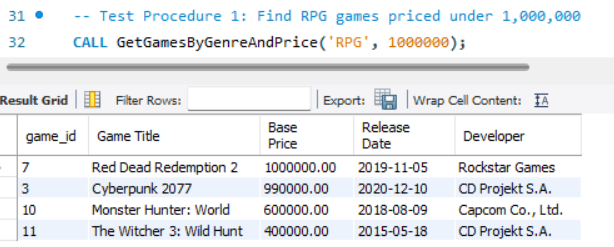
\includegraphics[width=0.9\linewidth]{graphics/get_games_by_genre_price_result.png}
    \caption{Result of retrieving RPG games priced under 1,000,000}
    \label{fig:get-games-by-genre-price-result}
\end{figure}

\begin{figure}[H]
    \centering
    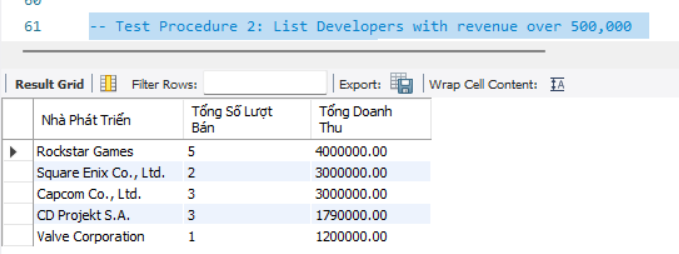
\includegraphics[width=0.9\linewidth]{graphics/get_developer_revenue_result.png}
    \caption{Result of retrieving developers with revenue over 500,000}
    \label{fig:get-developer-revenue-result}
\end{figure}